\documentclass[tikz,border=10pt]{standalone}
\usepackage{amsmath}
\begin{document}
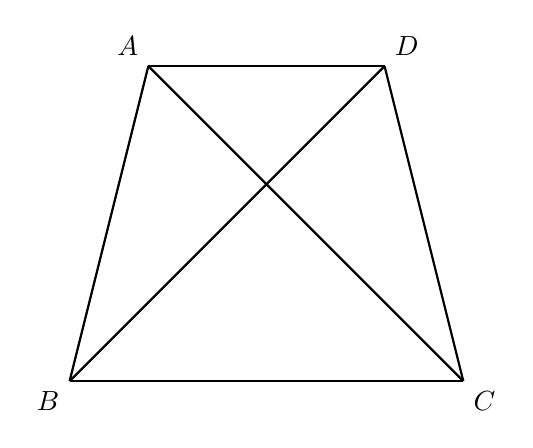
\begin{tikzpicture}[thick, scale=1]
  \coordinate (A) at (0,0);
  \coordinate (D) at (3,0);
  \coordinate (B) at (-1,-4);
  \coordinate (C) at (4,-4);

  \draw (A) -- (D);
  \draw (B) -- (A);
  \draw (D) -- (C);
  \draw (B) -- (C);
  \draw (B) -- (D);
  \draw (A) -- (C);

  \node[above left] at (A) {$A$};
  \node[above right] at (D) {$D$};
  \node[below left] at (B) {$B$};
  \node[below right] at (C) {$C$};
\end{tikzpicture}
\end{document}
